\chapter{Neural Language Models}

In this chapter, we introduce the notation used throughout the thesis and give a brief overview of the development of neural language models (NLM). We also review some of the main weaknesses shown by this family of models and how they have been addressed in the literature. 

\section{Notation}
\label{sec:notation}

Before continuing, we will define the notation used in the thesis:

\begin{itemize}
	\item Scalars are denoted with lowercase letters, such as $x$.
	
	\item Vectors are denoted with bold lowercase letters, such as $\mathbf{x}$ with $\mathbf{x}_i$ its $i$-th element, and are always assumed to be column vectors.
	
	\item Matrices are denoted with uppercase letters, such as $X$ with $X_{ij}$ its $(i,j)$-th element, $X_{i,:}$ its $i$-th row and $X_{:,j}$ its $j$-th column.
\end{itemize}

\section{Background}
\label{sec:background}

Prior to introducing the specifics of NLMs, we will formalize the task at hand and introduce some of its core concepts. 

\subsection{Language Modeling}

First, we define a \textbf{word-based language model} as a model able to compute the probability of a sentence or sequence of words $p(w_1, \ldots ,w_n)$. Such models are of great use in tasks where we have to recognize words in noisy or ambiguous input such as speech recognition or machine translation, among others.

If we now decompose the joint probability of a sequence using the chain rule of probability as shown in \autoref{eq:lm}, we observe that the function that needs to be estimated boils down to the conditional probability of a word given the history of previous words. However, taking into account the whole context poses a problem as language is creative and any particular sequence might have occurred few (or no) times before.  Many of the models that we will introduce approximate the true conditional distribution by making a Markov assumption as shown in \autoref{eq:markov}. This means that the probability of an upcoming word is fully characterized by the previous $n-1$ words. Despite seeming an incorrect premise for a complex source of information such as language, it has been proven to work really well in practice.

\begin{equation} \label{eq:lm}
	\begin{gathered}
		p(w_1, \ldots ,w_n)=p(w_1)p(w_2|w_1)p(w_3|w_{1}^{2}) \ldots p(w_n|w_{1}^{n-1}) \\
		= \prod_{k=1}^{n} p(w_k|w_{1}^{k-1})
	\end{gathered}
\end{equation}

\begin{equation} \label{eq:markov}
	p(w_k|w_{1}^{k-1}) \approx p(w_k|w_{k-1}^{k-n})
\end{equation}

\subsection{Evaluation}

Following a common practice in machine learning, we use a test set in order to evaluate our models. In the case of language modeling we have a word sequence $W_1^n=\{w_1, \ldots , w_n\}$ and we expect the model to assign it a high probability. Rather than working directly with raw probabilities we define a metric called \textbf{perplexity}, which is the geometric average of the inverse of the probability over the test set, as shown in \autoref{eq:pp}. Therefore, lower perplexity is better.

\begin{equation} \label{eq:pp}
	\begin{gathered}
		\text{Perplexity}(W_1^n) = p(W_1^n)^{-\frac{1}{n}} = \sqrt[n]{\frac{1}{p(W_1^n)}} \\
		= \sqrt[n]{\frac{1}{\prod_{k=1}^{n} p(w_k|W_{1}^{k-1})}}
	\end{gathered}
\end{equation}

Moreover, we can regard language as an information source and therefore use Information Theory to find a different (and equivalent) interpretation of perplexity. For that we need to introduce the basic concept of \textbf{entropy} (\autoref{eq:entropy} shows its formulation for discrete variables), which measures the expected uncertainty or ``surprise" $S$ of the value of a random variable $X$. Without going into details, it is easy to see that defining uncertainty as the negative logarithm (the specific base doesn't matter, but traditionally it is assumed to be 2) of the probability of each event matches our intuition (like $S(p)>S(q) \ \text{then} \ p<q$).

\begin{equation} \label{eq:entropy}
	H(X)=\mathbb{E}[S(X)]=-\sum_{x \in \mathcal{X}}p(x)\log_2(p(x)) \quad \text{with} \quad S(\cdot)=-\log_2(\cdot)
\end{equation}

A difference when it comes to language is that it involves dealing with sequences $W_1^n$ of discrete random variables. For a given language $L$ we can define the entropy of a variable ranging over all possible sequences of length $n$. To obtain the entropy-per-word we only need to normalize by $n$ (\autoref{eq:entropySeq}).

\begin{equation} \label{eq:entropySeq}
	\frac{1}{n} H(W_1^n) = -\frac{1}{n}\sum_{W_1^n \in L}p(W_1^n)\log_2(p(W_1^n))
\end{equation}

Additionally, in order to calculate the true entropy of a language we would need to consider sequences of infinite length (\autoref{eq:trueEntropySeq}). Fortunately, the Shannon-McMillan-Breiman theorem states that if a stochastic source (such as language) is regular in certain ways (stationary and ergodic) we can take a single long enough sequence instead of summing over all possible sequences (* in \autoref{eq:trueEntropySeq}).

\begin{equation} \label{eq:trueEntropySeq}
	\begin{gathered}
		H(L) = -\lim\limits_{n \rightarrow \infty}\frac{1}{n}\sum_{W_1^n \in L}p(W_1^n)\log_2(p(W_1^n))\\
		\stackrel{*}{=} -\lim\limits_{n \rightarrow \infty}\frac{1}{n}\log_2(p(W_1^n))
	\end{gathered}
\end{equation}

Related to the concept of entropy we have \textbf{cross-entropy}, which measures the relative entropy of $p$ with respect to $m$, $p$ being the true probability distribution and $m$ a model (e.g. an approximation) of $p$ over the same underlying set of events. After applying the Shannon-McMillan-Breiman theorem and assuming that $n$ is large enough, we can see in \autoref{eq:crossEntropy} the final formulation of the cross-entropy, which has become the standard loss function when optimizing neural language models.

\begin{equation} \label{eq:crossEntropy}
	\begin{gathered}
		H(p,m) = -\lim\limits_{n \rightarrow \infty}\frac{1}{n}\sum_{W_1^n \in L}p(W_1^n)\log_2(m(W_1^n)) \\
		\stackrel{*}{=} -\lim\limits_{n \rightarrow \infty}\frac{1}{n}\log_2(m(W_1^n)) \approx -\frac{1}{n}\log_2(m(W_1^n)) \\
		= -\frac{1}{n}\sum_{k=1}^{n}\log_2(m(w_k|W_{1}^{k-1}))
	\end{gathered}
\end{equation}

Finally, we can see in \autoref{eq:relationCrossAndPP} how cross-entropy and perplexity are connected. This relation gives raise to a nice interpretation of perplexity as branching factor: entropy measures uncertainty (in bits, if we use $\log_2$) but in exponentiated form it is measured as the cardinality of a uniform distribution with equivalent uncertainty.

\begin{equation} \label{eq:relationCrossAndPP}
	\text{Perplexity}(W_1^n) = 2^{H(p,m)} = m(W_1^n)^{-\frac{1}{n}}
\end{equation}

\section{Feed-Forward Neural Network Language Models \\ (FFNNLM)}
\label{sec:forwardnlm}

Until the appearance of NLMs, the most successful approaches were based on n-grams, which are models that estimate words from a fixed window of previous words and estimate probabilities by counting in a corpus and normalizing. Due to their nature, n-gram estimates intrinsically suffer from sparsity and several methods like smoothing, backoff and interpolation have been proposed to deal with this problem \cite{chen1996empirical}.

Along those lines, the first successful attempt of applying neural networks to language modeling \cite{bengio2003neural} remarked the effect of the \textit{curse of dimensionality} when it comes to estimating the joint distribution of many discrete random variables (such as words in a sentence). On the contrary, by using continuous variables we obtain better generalization because the function to be learned can be expected to have some local smoothness properties (``similar" words should get similar probabilities of being predicted). While requiring to be trained (n-grams don't), this approach is able to achieve significantly better results (reductions between 10\% and 20\% in perplexity with respect to a smoothed trigram model) by jointly learning word representations and a statistical language model.

Similar to n-grams, the model introduced in \cite{bengio2003neural} conditions the probability of a word on the previous $n-1$ words. The main difference lies in the concept of \textbf{distributed feature vectors}; words are embedded into a vector-space by assigning them a real vector representation of size $m$ via a look-up operation over the embedding matrix $C$ as shown in \autoref{eq:fwnlm}. 

\begin{equation} \label{eq:fwnlm}
	\begin{gathered}
		\mathbf{x} = [C_{w_{t-1},:} \, ; C_{w_{t-2},:} \, ; \cdots \, ; C_{w_{t-n+1},:})] \\
		\mathbf{y} = W\mathbf{x} + U \tanh(H\mathbf{x}+\mathbf{d}) + \mathbf{b} \\
		\mathbf{\hat{p}}_i=\hat{p}(w_t=i|w_{t-1},\ldots,w_{t-n+1}) = \frac{e^{\mathbf{y}_i}}{\sum_{n}e^{\mathbf{y}_n}} \\
	\end{gathered}
\end{equation}

where $[\;]$ is the concatenation operator, $C \in \mathbb{R}^{|V| \times m}$, $\mathbf{x} \in \mathbb{R}^{1 \times (n-1)m}$, $W \in \mathbb{R}^{|V| \times (n-1)m}$, $U \in \mathbb{R}^{|V| \times h}$, $H \in \mathbb{R}^{h \times (n-1)m}$, $\mathbf{d} \in \mathbb{R}^{h}$ and $\mathbf{y} ,\mathbf{b} \in \mathbb{R}^{|V|}$. 

The concatenated word representations $\mathbf{x}$ are fed through one (or more) nonlinear hidden layer (weights $H$ and bias $\mathbf{d}$), resulting in a hidden representation of size $h$. We then apply an affine transformation (weights $U$ and bias $\mathbf{b}$) to this hidden representation to obtain $\mathbf{y}$, an unnormalized probability distribution over the vocabulary $V$. Optionally, we can include direct connections from the word features to the output ($W$). Finally, a softmax operation produces a valid probability distribution over the full vocabulary.

\begin{figure}[H]
	\centering
	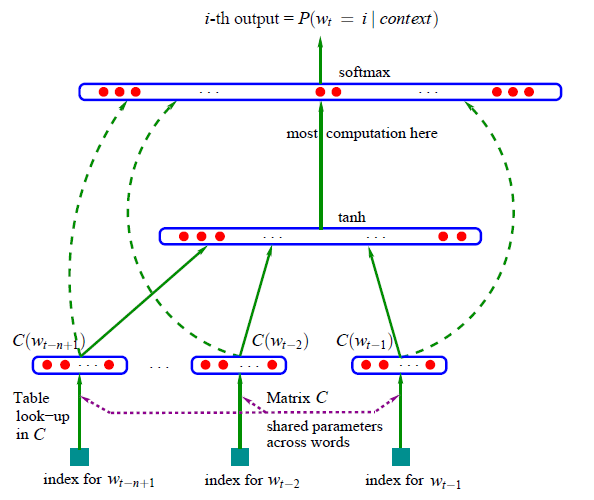
\includegraphics[scale=0.5]{fflm}
	\captionof{figure}{Feed-Forward NLM architecture \cite{bengio2003neural}}
	\label{fig:ffarch}
\end{figure}

Having a look at the full model (shown in \autoref{fig:ffarch}) we can observe that most expensive operation is the computation of the unnormalized probability distribution $\mathbf{y}$, which requires a number of dot products that scales linearly with $|V|$ (it is not unusual to work with vocabulary sizes in the order of the tens of thousands). 

Several practical solutions have been proposed to avoid it, with \textbf{hierarchical softmax} \cite{mnih2009scalable} being one of the most popular ones. It uses a hierarchical binary tree representation of the vocabulary with words as its leaves and, for each node, explicitly represents the relative probabilities of its child nodes. These define a random walk that assigns probabilities to words, allowing to reduce the complexity of obtaining the output probability of a single word to around $\log_2(|V|)$.

\section{Word Vectors}
\label{sec:wv}

As we stated in the previous section, distributed continuous vectors allow for ``clever" smoothing by taking into account syntactic and semantic features that are automatically learnt. \cite{mikolov2013efficient} picked up on this concept trying to find ways of training these vector representations more efficiently. The paper introduces a family of models known as \textbf{word2vec}, whose architecture matches the one from a FFNNLM where the nonlinear hidden layer has been removed (ending up with a simple log bilinear model). The difference between them lies on the objective they optimize for. It is important to note that these objectives are designed as a mean to learn meaningful word embeddings, which are the main focus of the following architectures:

\begin{itemize}
	\item Continuous Bag-of-Words model (CBOW): given a symmetric window of size $k$ around a specific position $i$ $\{w_{i-k}, \ldots , w_{i-1}, w_{i+1}, \ldots w_{i+k}\}$, we want to predict the word $w_i$. The term ``bag-of-words" comes from the fact that the embeddings of the whole window are summed (instead of concatenated) and thus, order is not preserved.
	
	\item Continuous Skip-Gram model: given a specific position $i$ we randomly sample words inside its surrounding window and try to predict them. Therefore, each training example is a 2-tuple consisting of $w_i$ as input and a sampled word from the window as output.
\end{itemize}

In addition to a simplified architecture and a modified objective, further optimizations for the Skip-Gram model were introduced in a follow-up paper \cite{mikolov2013distributed}. As we already explained at the end of the previous section, calculating a probability distribution over the full vocabulary is computation-intensive. In order to avoid doing this, the original task is casted into a binary classification problem by making use of a new objective named \textbf{negative sampling}. Inspired by noise contrastive estimation (NCE), the objective is to distinguish the target word $w_O$ from draws coming from a noise distribution $p_n(w)$ (e.g. unigram distribution) using logistic regression, where there are $k$ noise samples for each data point (\autoref{eq:ns}).

\begin{equation} \label{eq:ns}
	\begin{gathered}
		\mathcal{L}(\theta) = \log(\sigma(\mathbf{v_{w_O}}^{\top} \mathbf{v_{w_I}})) + \sum_{i=1}^{k} \log(-\sigma(\mathbf{v_{w_i}}^{\top} \mathbf{v_{w_I}})) \\ 
		\text{with} \quad w_i \sim p_n(w)
	\end{gathered}
\end{equation}

Another famous family of word vectors is \textbf{GloVe} \cite{pennington2014glove}, where the objective is a weighted (weighting function $f(\cdot)$) least squares fit of the log-counts (\autoref{eq:glove}). Rather than capturing co-occurences one word at a time (like word2vec), GloVe does dimensionality reduction on the whole co-occurrence counts matrix $N$. 

\begin{equation} \label{eq:glove}
	\mathcal{L}(\theta, N) = \sum_{i,j:N_{ij}>0}f(N_{ij})(\log(N_{ij})-(\mathbf{v_{w_O}}^{\top} \mathbf{v_{w_I}} + b_O + b_I))^2
\end{equation}

In general, word vectors have proven to excel at capturing semantic features. For example, \cite{mikolov2013efficient} analyzes how Skip-Gram vectors achieve very good results on the semantic word relationship task. Furthermore, the authors qualitatively explore how the resulting vector representations encode semantic information in the affine embedding structure. Hence, a vector operation like $\textit{Spain}-\textit{Madrid}+\textit{Switzerland}$ would lead to the desired answer $\textit{Bern}$.

In summary, word vectors have become a standard in NLP and are used as input in all sorts of downstream applications such as sentiment analysis.

\section{Recurrent Neural Network Language Models \\ (RNNLM)}
\label{sec:rnn}

So far all the models that we have seen (n-grams and FFNNLM) explicitly use a fixed length context. Recurrent neural networks remove this limitation by introducing recurrent connections that allow information to cycle for an arbitrarily long time (although this is not true in practice). They learn to compress the whole history in low dimensional space (hidden state $\mathbf{h}(t)$) that is sequentially updated by being blended with the current input $\mathbf{x}(t)$ (\autoref{eq:rnncell} introduces the formulation for Elman networks).

\begin{equation} \label{eq:rnncell}
		\mathbf{h}(t) = \sigma_h(W_h \mathbf{x}(t) + U_h \mathbf{h}(t-1) + \mathbf{b_h})
\end{equation}

where $W_h \in \mathbb{R}^{h \times m}$, $\mathbf{x}(t) \in \mathbb{R}^{m}$, $U_h \in \mathbb{R}^{h \times h} , \mathbf{h}(t), \mathbf{h}(t-1), \mathbf{b_h} \in \mathbb{R}^{h}$ and $\sigma_h$ is a nonlinear function (e.g. sigmoid). 

It is important to note that the network parameters are shared over time. \cite{mikolov2010recurrent} was one of the first to successfully apply RNNs to language modeling. The hidden states $\mathbf{h}(t)$ are fed through a fully connected layer to produce a probability distribution over the vocabulary in a similar way to FFNNLMs.

\begin{equation} \label{eq:rnnlm}
	\begin{gathered}
		\mathbf{y}(t) = W_y \mathbf{h}(t) + \mathbf{b_y} \\
		\mathbf{\hat{p}}(t)_i=\hat{p}(w_t=i|\mathbf{h}(t)) = \frac{e^{\mathbf{y}(t)_i}}{\sum_{n}e^{\mathbf{y}(t)_n}} \\
	\end{gathered}
\end{equation}

where $W_y \in \mathbb{R}^{|V| \times h}$ and $\mathbf{y}(t)$, $\mathbf{b_y}, \mathbf{\hat{p}}(t) \in \mathbb{R}^{|V|}$.

\subsection{Backpropagation Through Time (BPTT)}

Backpropagation is the standard gradient computation technique used for neural networks. However when applied to the recurrent connections of an RNN, the gradients will depend on the previous timesteps (up to $t=0$). Thus, we call Backpropagation Through Time (BPTT) \cite{werbos1990backpropagation} to the application of backpropagation on an unrolled RNN, which accounts for this dependencies by summing up the gradients for each time step. In \autoref{eq:bptt} we see an example of this when calculating the gradient for $U_h$.

\begin{equation} \label{eq:bptt}
	\frac{\partial \mathcal{L}(t)}{\partial U_h} = \frac{\partial \mathcal{L}(t)}{\partial \mathbf{\hat{p}}(t)}\frac{\partial \mathbf{\hat{p}}(t)}{\partial \mathbf{h}(t)}\frac{\partial \mathbf{h}(t)}{\partial U_h} = \sum_{k=0}^{t} \frac{\partial \mathcal{L}(t)}{\partial \mathbf{\hat{p}}(t)}\frac{\partial \mathbf{\hat{p}}(t)}{\partial \mathbf{h}(t)}\frac{\partial \mathbf{h}(t)}{\partial \mathbf{h}(k)}\frac{\partial \mathbf{h}(k)}{\partial U_h}
\end{equation}

One of the main problems of BPTT is the high cost of a single parameter update, which makes it impossible to use for large numbers of iterations. \textbf{Truncated Backpropagation Through Time} (TBPTT), which is a modified version of BPTT, was introduced in \cite{sutskever2013training} to work around this limitation. When using TBPTT, the sequence is processed one timestep at a time, and every $k_1$ timesteps, it runs BPTT for $k_2$ timesteps, so a parameter update can be cheap if $k_2$ is small. Most implementations assume $k_1=k_2$.

\subsection{Exploding and Vanishing Gradient}

The number of derivatives required for a single weight update is directly proportional to the number of steps of our input sequences. We can see this in \autoref{eq:gradient} by observing that the term $\frac{\partial \mathbf{h}(t)}{\partial \mathbf{h}(k)}$ is a chain-rule itself. Citing \cite{pascanu2013difficulty}, \textit{``a product of $t-k$ real numbers can shrink to zero or explode to infinity, so does this product of matrices"} and therefore, this can cause gradients to vanish or explode. 

\begin{equation} \label{eq:gradient}
	\frac{\partial \mathbf{h}(t)}{\partial \mathbf{h}(k)} = \prod_{t \geq i > k} \frac{\partial \mathbf{h}(i)}{\partial \mathbf{h}(i-1)}
\end{equation}

For exploding gradients, clipping the norm of the gradients to a pre-defined threshold has proven to be an effective remedy for this problem. Moreover, vanishing gradients translate into gradient contributions from ``far away" steps becoming zero, and thus hindering the learning of long-range dependencies. The most popular solution for this problem has been the introduction of new cell architectures explicitly designed to deal with vanishing gradients such as Long Short-Term Memory (LSTM) \cite{hochreiter1997long} and Gated Recurrent Units (GRU) \cite{cho2014learning}. We will focus on the LSTM as the GRU cell is just a simplified version of the former. The main differences to a vanilla RNN are the introduction of a cell state $\mathbf{c}(t)$ (that acts as internal memory) and the gates $\mathbf{f}(t)$, $\mathbf{i}(t)$ and $\mathbf{o}(t)$: 

\begin{equation} \label{eq:lstmcell}
	\begin{gathered}
		\mathbf{f}(t) = \sigma_g(W_f \mathbf{h}(t-1) + U_f\mathbf{x}(t) + \mathbf{b}_f) \\
		\mathbf{i}(t) = \sigma_g(W_i \mathbf{h}(t-1) + U_i \mathbf{x}(t) + \mathbf{b}_i) \\
		\mathbf{o}(t) = \sigma_g(W_o \mathbf{h}(t-1) + U_o \mathbf{x}(t) + \mathbf{b}_o) \\
		\mathbf{\tilde{c}}(t) = \sigma_c(W_c \mathbf{h}(t-1) + U_c \mathbf{x}(t) + \mathbf{b}_c) \\
		\mathbf{c}(t) = \mathbf{f}(t) \odot \mathbf{c}(t-1) + \mathbf{i}(t) \odot \mathbf{\tilde{c}}(t) \\
		\mathbf{h}(t) = \mathbf{o}(t) \odot \sigma_h(\mathbf{c}(t))\\
	\end{gathered}
\end{equation}

where $W_f,W_i,W_o,W_f \in \mathbb{R}^{h \times h}$, $U_f,U_i,U_o,U_f \in \mathbb{R}^{h \times m}$, $\mathbf{f}(t),\mathbf{b}_f,\mathbf{i}(t),\mathbf{b}_i,  \allowbreak \mathbf{o}(t),\mathbf{b}_o,\mathbf{c}(t),\mathbf{b}_c,\mathbf{\tilde{c}}(t) \in \mathbb{R}^{h}$ and $\sigma_g,\sigma_c,\sigma_h$ are non linear functions. 

Gates are a way to optionally let information through and are learnt in such a way that the cell can remember long-range dependencies. Each gate is calculated as an affine transformation of the current input $\mathbf{x}(t)$ and the previous hidden state $\mathbf{h}(t-1)$ followed by a non linearity, as shown in \autoref{eq:lstmcell}. These gates modify the cell state through pointwise multiplications; specifically, the new cell state is formed by a combination of the previous cell state weighted by the forget gate $\mathbf{f}(t)$ and the ``newly proposed" state $\mathbf{\tilde{c}}(t)$ weighted by the input gate $\mathbf{i}(t)$. Therefore, gates provide an explicit way for the cell to decide what information should be forgotten and what is worth remembering for the next steps.  

\begin{figure}[H]
	\centering
	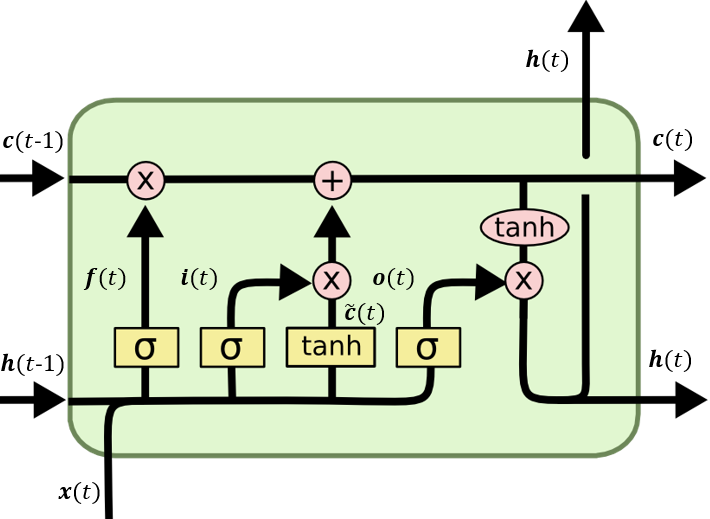
\includegraphics[scale=0.6]{lstm_cell}
	\captionof{figure}{LSTM cell architecture \cite{colah2015lstm}}
	\label{fig:ffarch}
\end{figure}

To sum up, recurrent neural network architectures using LSTM cells have become ubiquitous in a wide range of NLP tasks and are a key element for state-of-the-art language models \cite{jozefowicz2016exploring}.